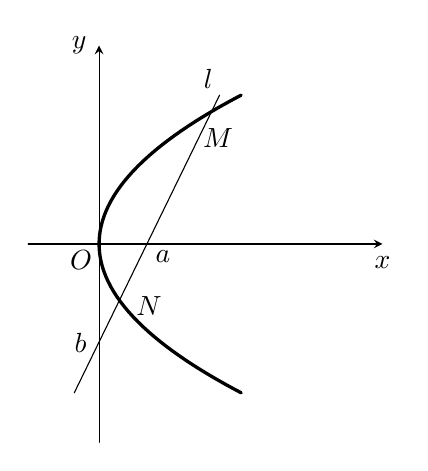
\begin{tikzpicture}[>=stealth, scale=0.9, line cap=round, line join=round]
  % Axes
  \draw[->] (-1.0, 0) -- (4.0, 0) node[below=1pt] {$x$};
  \draw[->] (0, -2.8) -- (0, 2.8) node[left=1pt] {$y$};
  \node[below left=-1pt] at (0, 0) {$O$};

  % Parabola x = y^2 / 2.5
  \draw[very thick] plot[domain=-2.1:2.1, samples=60] ({(\x)^2 / 2.2}, \x);

  % Line l intersecting at M (approx y=1.4) and N (approx y=-0.8)
  % Points: M = (1.4^2/2.2, 1.4) = (0.89, 1.4)
  % N = ((-0.8)^2/2.2, -0.8) = (0.29, -0.8)
  % Slope = (1.4 - (-0.8)) / (0.89 - 0.29) = 2.2 / 0.6 = 3.67
  \draw (-0.35, -2.1) -- (1.7, 2.1) node[above left=-1pt] {$l$};

  % Intersections
  \coordinate (M) at (1.37, 1.73);
  \coordinate (N) at (0.35, -0.88);

  % Axis intercepts
  \node[below right=-1pt] at (0.7, 0) {$a$};
  \node[left=1pt] at (0, -1.4) {$b$};

  % Labels
  \node[below right=-1pt] at (1.37, 1.73) {$M$};
  \node[right=1pt] at (0.35, -0.88) {$N$};
\end{tikzpicture}
